% !TeX root = 机械设计.tex
% ============================================================
%  第五章 轴毂连接
%  来源：课件《05轴毂连接》与《4.轴毂连接.md》笔记整理
% ============================================================
\chapter{轴毂连接}
\label{chap:轴毂连接}

\section{键连接的类型及应用}
\label{sec:键连接类型}

根据键连接在装配时是否预紧，分为\textbf{松键连接}和\textbf{紧键连接}：
\begin{equation}
	\text{松键连接}\ \begin{cases}
		\text{平键连接}\ \begin{cases}
			\text{普通平键}\\
			\text{导向平键}\\
			\text{滑键}
		\end{cases}\\[2pt]
		\text{半圆键连接}
	\end{cases}
	\label{eq:轴毂:松键连接}
\end{equation}
\begin{equation}
	\text{紧键连接}\ \begin{cases}
		\text{楔键连接}\\
		\text{切向键连接}
	\end{cases}
	\label{eq:轴毂:紧键连接}
\end{equation}

\begin{figure}[htbp]
	\centering
	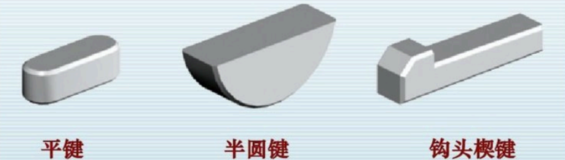
\includegraphics[width=0.9\textwidth]{Figure/几种键.png}
	\caption{几种键}
	\label{fig:轴毂:几种键}
\end{figure}

\subsection{平键}
\label{sec:平键}

工作面：两侧面；工作时靠键与键槽侧面的挤压来传递扭矩。

\subsubsection{普通平键}

用于静连接，即轴与轮毂之间无相对轴向移动。
\begin{figure}[htbp]
	\centering
	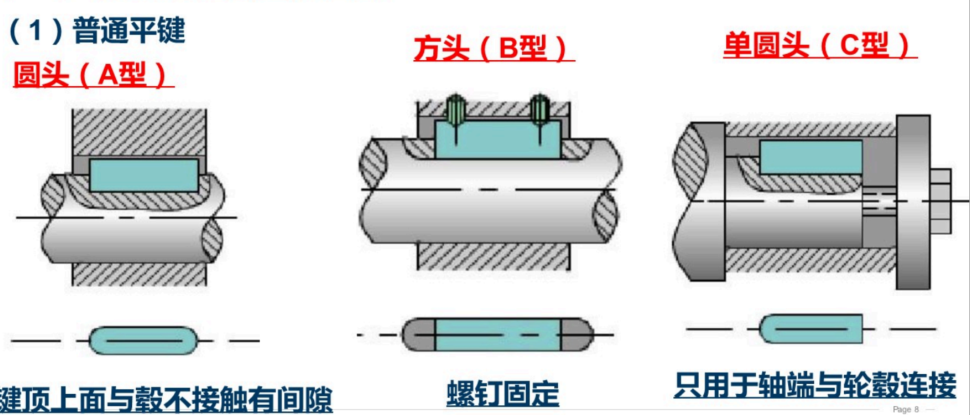
\includegraphics[width=0.85\textwidth]{Figure/普通平键.png}
	\caption{普通平键}
	\label{fig:轴毂:普通平键}
\end{figure}

\subsubsection{薄型平键}

键高约为普通平键的 $60\%\sim70\%$；有圆头、方头和单圆头，常用于薄壁结构、空心轴等径向尺寸受限制的场合。

\subsubsection{导向键和滑键}

\begin{figure}[htbp]
	\centering
	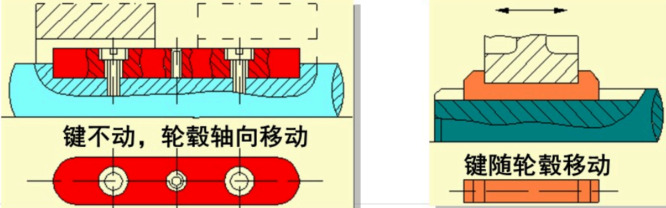
\includegraphics[width=0.8\textwidth]{Figure/导向键和滑键.png}
	\caption{导向键和滑键}
	\label{fig:轴毂:导向键和滑键}
\end{figure}

\subsection{半圆键连接}
\label{sec:半圆键}

\begin{figure}[htbp]
	\centering
	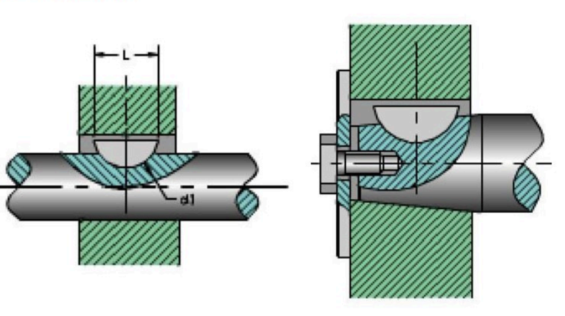
\includegraphics[width=0.55\textwidth]{Figure/半圆键.png}
	\caption{半圆键连接}
	\label{fig:轴毂:半圆键}
\end{figure}

键槽用与半圆键形状相同的铣刀加工，键能在槽中绕几何中心摆动，工作时靠工作侧面的挤压传递扭矩。

\begin{note}
半圆键要注意画法：
\begin{enumerate}
	\item 半圆键的两侧面为键的工作面，只在接触面上画一条轮廓线；
	\item 应画出键上表面与轮毂的间隙。
\end{enumerate}
\begin{figure}[htbp]
	\centering
	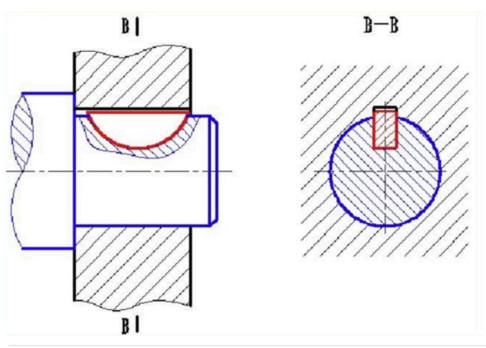
\includegraphics[width=0.5\textwidth]{Figure/半圆键连接画法.png}
	\caption{半圆键连接的画法}
	\label{fig:轴毂:半圆键画法}
\end{figure}
\end{note}

\subsection{楔键连接}
\label{sec:楔键}

键的上表面与轮毂键槽底均具有 $1:100$ 的斜度，工作时键的上下表面与轮毂、轴的键槽工作面压紧，靠摩擦力和挤压传递扭矩。

\begin{figure}[htbp]
	\centering
	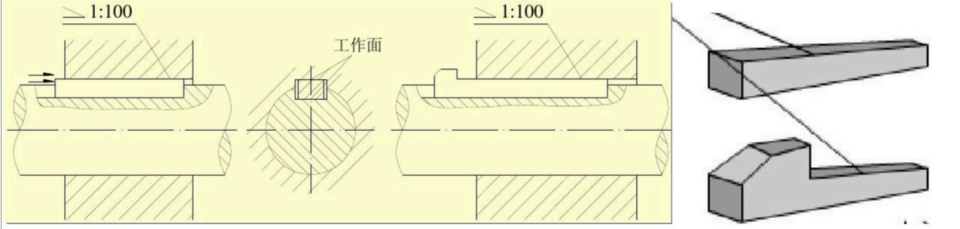
\includegraphics[width=0.9\textwidth]{Figure/楔键连接.png}
	\caption{楔键连接（普通楔键和钩头楔键）}
	\label{fig:轴毂:楔键}
\end{figure}

楔紧后，轴和轮毂产生偏心，在冲击载荷下易松脱，仅适用于低速轻载、精度要求不高的场合。

\subsection{切向键}
\label{sec:切向键}

切向键由两个普通的楔键组成，靠上下表面与键槽底面的挤压力和轮毂接触的摩擦力传递扭矩。适用于精度要求不高，低速、重载，轴径大于 $100$ mm 的轴上。

\begin{figure}[htbp]
	\centering
	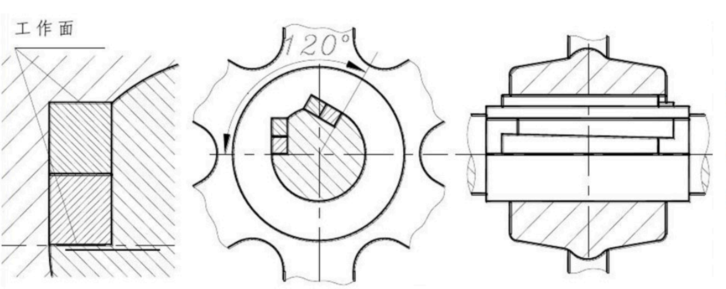
\includegraphics[width=0.7\textwidth]{Figure/切向键.png}
	\caption{切向键}
	\label{fig:轴毂:切向键}
\end{figure}

\section{键的选择和键连接的强度计算}
\label{sec:键的选择和强度计算}

\subsection{键的类型选择}
\label{sec:键的类型选择}

\begin{table}[H]
\centering
\small
\setlength{\tabcolsep}{4pt}
\caption{键的类型选择}
\label{tab:轴毂:键的类型}
\begin{tabular}{p{1.5cm}p{4.1cm}p{4.5cm}p{4.1cm}}
	\toprule
	键的名称 & 使用要求 & 结构特点 & 工作条件 \\
	\midrule
	普通平键 & 用于静连接，轴与轮毂之间无相对轴向移动 & 矩形截面，两侧面为工作面；有圆头、方头、单圆头三种型式 & 靠键与键槽侧面的挤压传递扭矩 \\
	薄型平键 & 用于薄壁结构、空心轴等径向尺寸受限制的场合 & 键高约为普通平键的 $60\%\sim70\%$；有圆头、方头和单圆头 & 同普通平键，靠两侧面的挤压传递扭矩 \\
	导向平键 & 用于轮毂需沿轴作轴向移动的动连接，移动距离一般不大 & 键固定在轴上，轮毂可沿键滑动 & 靠两侧面挤压传递扭矩，兼起导向作用 \\
	滑键 & 用于轮毂沿轴移动距离较大的动连接 & 键固定在轮毂上，随轮毂一起沿轴上较长的键槽滑动 & 靠两侧面挤压传递扭矩，随轮毂一起移动 \\
	半圆键 & 适用于锥形轴端及传递较小扭矩的场合（轴槽较深，对轴的强度削弱较大） & 呈半圆形，键能在轴槽中绕几何中心摆动；键槽用与键形状相同的铣刀加工 & 靠工作侧面（两侧面）的挤压传递扭矩 \\
	楔键 & 仅适用于低速、轻载、精度要求不高的场合 & 键的上表面与轮毂键槽底均具有 $1:100$ 的斜度，工作时上下表面压紧 & 靠上下表面的挤压力和摩擦力传递扭矩；楔紧后轴与轮毂产生偏心，在冲击载荷下易松脱 \\
	切向键 & 适用于精度要求不高、低速、重载、轴径大于 $100$ mm 的轴 & 由两个普通楔键组成 & 靠上下表面与键槽底面的挤压力和轮毂接触的摩擦力传递扭矩 \\
	\bottomrule
\end{tabular}
\end{table}

\subsection{键的尺寸选择}
\label{sec:键的尺寸选择}

键的尺寸关注两个量：截面尺寸（$b\times h$）和长度（$L$）。按轴的直径 $d$ 由标准选定截面尺寸，由轮毂长度确定键的长度。一般取键长\textbf{略短}于轮毂长度 $5\sim10$ mm。

\subsection{普通平键的强度计算}
\label{sec:平键强度}

假定载荷在键的工作面上均匀分布，普通平键的连接强度条件为
\begin{equation}
	\sigma_p=\frac{2T\times10^{3}}{kld}\le[\sigma]_p
	\label{eq:轴毂:平键挤压强度}
\end{equation}
其中：
\begin{itemize}
	\item $k$：键与轮毂的接触高度，$k=0.5h$，$h$ 为键的高度；
	\item $l$：键的工作长度，A 型键 $l=L-b$，B 型键 $l=L$，C 型键 $l=L-b/2$。
\end{itemize}

\subsection{导向键和滑键连接强度计算}
\label{sec:导向键强度}

导向键和滑键连接强度条件为
\begin{equation}
	p=\frac{2T\times10^{3}}{kld}\le[p]
	\label{eq:轴毂:导向键比压}
\end{equation}

\subsection{半圆键的剪切强度条件}
\label{sec:半圆键强度}

半圆键的剪切强度条件为
\begin{equation}
	T=N\cdot\frac{d}{2}\times10^{3}\approx bl\tau\cdot\frac{d}{2}\times10^{3}
	\label{eq:轴毂:半圆键转矩}
\end{equation}
\begin{equation}
	\tau=\frac{2000T}{bld}\le[\tau]
	\label{eq:轴毂:半圆键剪切}
\end{equation}
其中：
\begin{itemize}
	\item $\tau$：键剪切应力；
	\item $b$：键宽；
	\item $l$：键的工作长度，取 $l=L$。
\end{itemize}

\begin{note}
强度不足时：
\begin{enumerate}
	\item 当强度不足时，可适当增加键长或采用两个键按 $180^{\circ}$ 布置；
	\item 考虑两个键的载荷分布不均匀性，在强度校核时按 1.5 个键计算。
\end{enumerate}
\end{note}

\section{花键连接}
\label{sec:花键连接}

\subsection{花键连接的类型、特点及应用}
\label{sec:花键类型}

花键连接是由周向均匀分布的多个纵向键齿的\textbf{花键轴}和带有键槽的轮毂相配合构成的可拆连接。

\begin{definition}[花键连接的优缺点]
\label{def:花键优缺点}
\textbf{优点}：
\begin{enumerate}
	\item 键齿数多，总接触面积大，比平键承载能力高；
	\item 键齿与轴一体且槽较浅，齿根应力集中较小，对轴的削弱小；
	\item 键齿对称布置、均匀分布，受力均匀。
\end{enumerate}

\textbf{缺点}：结构相对复杂，加工时需要专门的刀具和设备，成本高。
\end{definition}

按齿形不同，花键连接分为\textbf{矩形花键}和\textbf{渐开线花键}：
\begin{itemize}
	\item 矩形花键——\textbf{内径定心}，定心精度高，定心稳定性好，可用磨削消除热处理后的变形；
	\item 渐开线花键——\textbf{齿形定心}，齿受载时齿上的径向力能自动定心，有利于各齿均载。
\end{itemize}

\subsection{花键连接的强度计算}
\label{sec:花键强度}

设计步骤：按轴径确定花键尺寸，再校核连接强度。

失效形式：压溃（静连接）、磨损（动连接）、齿根剪断。

假定工作载荷沿键的工作长度均匀分布，各齿面上压力的合力 $N$ 作用在平均直径 $d_m$ 处，即传递的转矩为
\begin{equation}
	T=\frac{Nd_m}{2}
	\label{eq:轴毂:花键转矩}
\end{equation}
静连接的挤压强度条件为
\begin{equation}
	\sigma_p=\frac{2T\times10^{3}}{\psi zhl d_m}\le[\sigma_p]
	\label{eq:轴毂:花键挤压强度}
\end{equation}
动连接的强度条件（耐磨性）为
\begin{equation}
	p=\frac{2T\times10^{3}}{\psi zhl d_m}\le[p]
	\label{eq:轴毂:花键耐磨性}
\end{equation}
其中：
\begin{itemize}
	\item $\psi$：载荷分配不均系数，$\psi=0.7\sim0.8$；
	\item $z$：花键的键齿数；
	\item $h$：花键齿侧面的高度；
	\begin{itemize}
		\item 矩形花键：$h=\dfrac{D-d}{2}-2C$（$D$ 为花键大径，$d$ 为花键小径，$C$ 为倒角尺寸）；
		\item 渐开线花键：$\alpha=30^{\circ}$ 时 $h=m$；$\alpha=45^{\circ}$ 时 $h=0.8m$。
	\end{itemize}
	\item $l$：键的工作长度；
	\item $d_m$：平均直径。
\end{itemize}

\section{无键连接}
\label{sec:无键连接}

轴与毂的连接不用键或花键时，统称无键连接。

\begin{definition}[型面连接（Profile connection）]
\label{def:型面连接}
轴与毂孔可为柱形或锥形。

特点：没有应力集中源，对中性好，承载能力强，装拆方便；但加工需用专用设备，应用较少。
\end{definition}

\begin{definition}[胀紧连接]
\label{def:胀紧连接}
利用锥面贴合并挤紧在轴毂之间，靠摩擦力传递扭矩。

特点：可传递较大的扭矩和轴向力，应力集中较小，对中性好，承载能力高，有过载保护作用；但轴毂之间需安装胀套，应用受到尺寸限制。
\end{definition}

\section{销连接}
\label{sec:销连接}

\begin{definition}[销按用途分类]
\label{def:销按用途}
\begin{itemize}
	\item \textbf{定位销}：主要用于零件间的位置定位，常用作组合加工和装配时的主要辅助零件；
	\item \textbf{连接销}：主要用于零件间的联接或锁定，可传递不大的载荷；
	\item \textbf{安全销}：主要用于安全保护装置中的过载剪断元件。
\end{itemize}
\end{definition}

\begin{definition}[销按结构形式分类]
\label{def:销按结构}
\begin{itemize}
	\item \textbf{圆柱销}：不宜多次装拆，否则定位精度下降；
	\item \textbf{圆锥销}：$1:50$ 锥度，可自锁，定位精度较高，允许多次装拆，且便于拆卸；
	\item \textbf{特殊型式销}：带螺纹锥销、开尾圆锥销、弹性销、开口销、槽销等。
\end{itemize}

销的常用材料为 35、45 钢。
\end{definition}

\section*{本章重点}
\addcontentsline{toc}{section}{本章重点}

\begin{enumerate}
	\item 松键和紧键的区别；
	\item 键大小的选择；
	\item 平键的挤压和剪切强度校核，强度不足时的措施；
	\item 花键的优缺点；
	\item 花键的类型。
\end{enumerate}
